\documentclass[aspectratio=169]{beamer}
\usepackage[english]{babel}
\usepackage{amsmath}
\usepackage[UTF8]{ctex}
\usepackage{cite}
% 加导航条
\useoutertheme[width=2.9\baselineskip,right]{sidebar}
% 目录标数字
\setbeamertemplate{section in toc}[sections numbered]
% 无序列表用实心点
\setbeamertemplate{itemize item}{$\bullet$}
% 设置每页标题格式
\setbeamertemplate{frametitle}
  {\vspace{-0.5cm}
   \insertframetitle
   \vspace{-0.5cm}}
% 去掉下面没用的导航条
\setbeamertemplate{navigation symbols}{}
% 设置页脚格式
\makeatother
\setbeamertemplate{footline}
{
  \leavevmode%
  \hbox{%
  \begin{beamercolorbox}[wd=.4\paperwidth,ht=2.25ex,dp=1ex,center]{author in head/foot}%
    \usebeamerfont{author in head/foot}\insertshortauthor
  \end{beamercolorbox}

  \begin{beamercolorbox}[wd=.6\paperwidth,ht=2.25ex,dp=1ex,center]{title in head/foot}%
    \usebeamerfont{title in head/foot}\insertshorttitle\hspace*{13em}
    \insertframenumber{} / \inserttotalframenumber\hspace*{0ex}
  \end{beamercolorbox}}

  \vskip0pt%
}
%设置脚注字号
\setbeamerfont{footnote}{size=\zihao{7}}
\makeatletter


% 定义颜色
\definecolor{alizarin}{rgb}{0.82, 0.1, 0.26} % 红色
\definecolor{DarkFern}{HTML}{407428} % 绿色
%\colorlet{main}{DarkFern!100!white} % 第一种设置方法
\colorlet{main}{red!70!black} % 第二种设置方法
\definecolor{bistre}{rgb}{0.24, 0.17, 0.12} % 黑色
\definecolor{mygrey}{rgb}{0.52, 0.52, 0.51} % 灰色
%\colorlet{main}{green!50!black}
\colorlet{text}{bistre!100!white}

% 不同元素指定不同颜色,fg是本身颜色,bg是背景颜色,!num!改变数值提供渐变色
\setbeamercolor{title}{fg=main}
\setbeamercolor{frametitle}{fg=main}
\setbeamercolor{section in toc}{fg=text}
\setbeamercolor{normal text}{fg=text}
\setbeamercolor{block title}{fg=main,bg=mygrey!14!white}
\setbeamercolor{block body}{fg=black,bg=mygrey!10!white}
\setbeamercolor{qed symbol}{fg=main} % 证明结束后的框颜色
\setbeamercolor{math text}{fg=black}
% 设置页脚对应位置颜色
\setbeamercolor{author in head/foot}{fg=black, bg=mygrey!5!white}
\setbeamercolor{title in head/foot}{fg=black, bg=mygrey!5!white}
\setbeamercolor{structure}{fg=main, bg=mygrey!10!white} % 设置sidebar颜色

% 左右页间距的排版
\def\swidth{2.3cm}
\setbeamersize{sidebar width right=\swidth}
\setbeamersize{sidebar width left=\swidth}
\setbeamerfont{title in sidebar}{size=\scriptsize}
\setbeamerfont{section in sidebar}{size=\tiny}


%-------------------正文-------------------------%

\author{邓志远}
\title{开题答辩}
\subtitle{局部紧的非Archimedean 域$F$上的退化$\mathfrak{P}$-adic群表示}
\date{\today}
\logo{
\includegraphics[width=1.3cm]{hui.jpeg}}
\begin{document}

\frame[plain]{\titlepage}

\begin{frame}
\frametitle{目录}
\tableofcontents
\end{frame}

\section{研究背景及其意义}

\frame{\frametitle{目录}\tableofcontents[currentsection]}

\begin{frame}
\frametitle{Langlands纲领的历史背景}

\begin{figure}[ht]
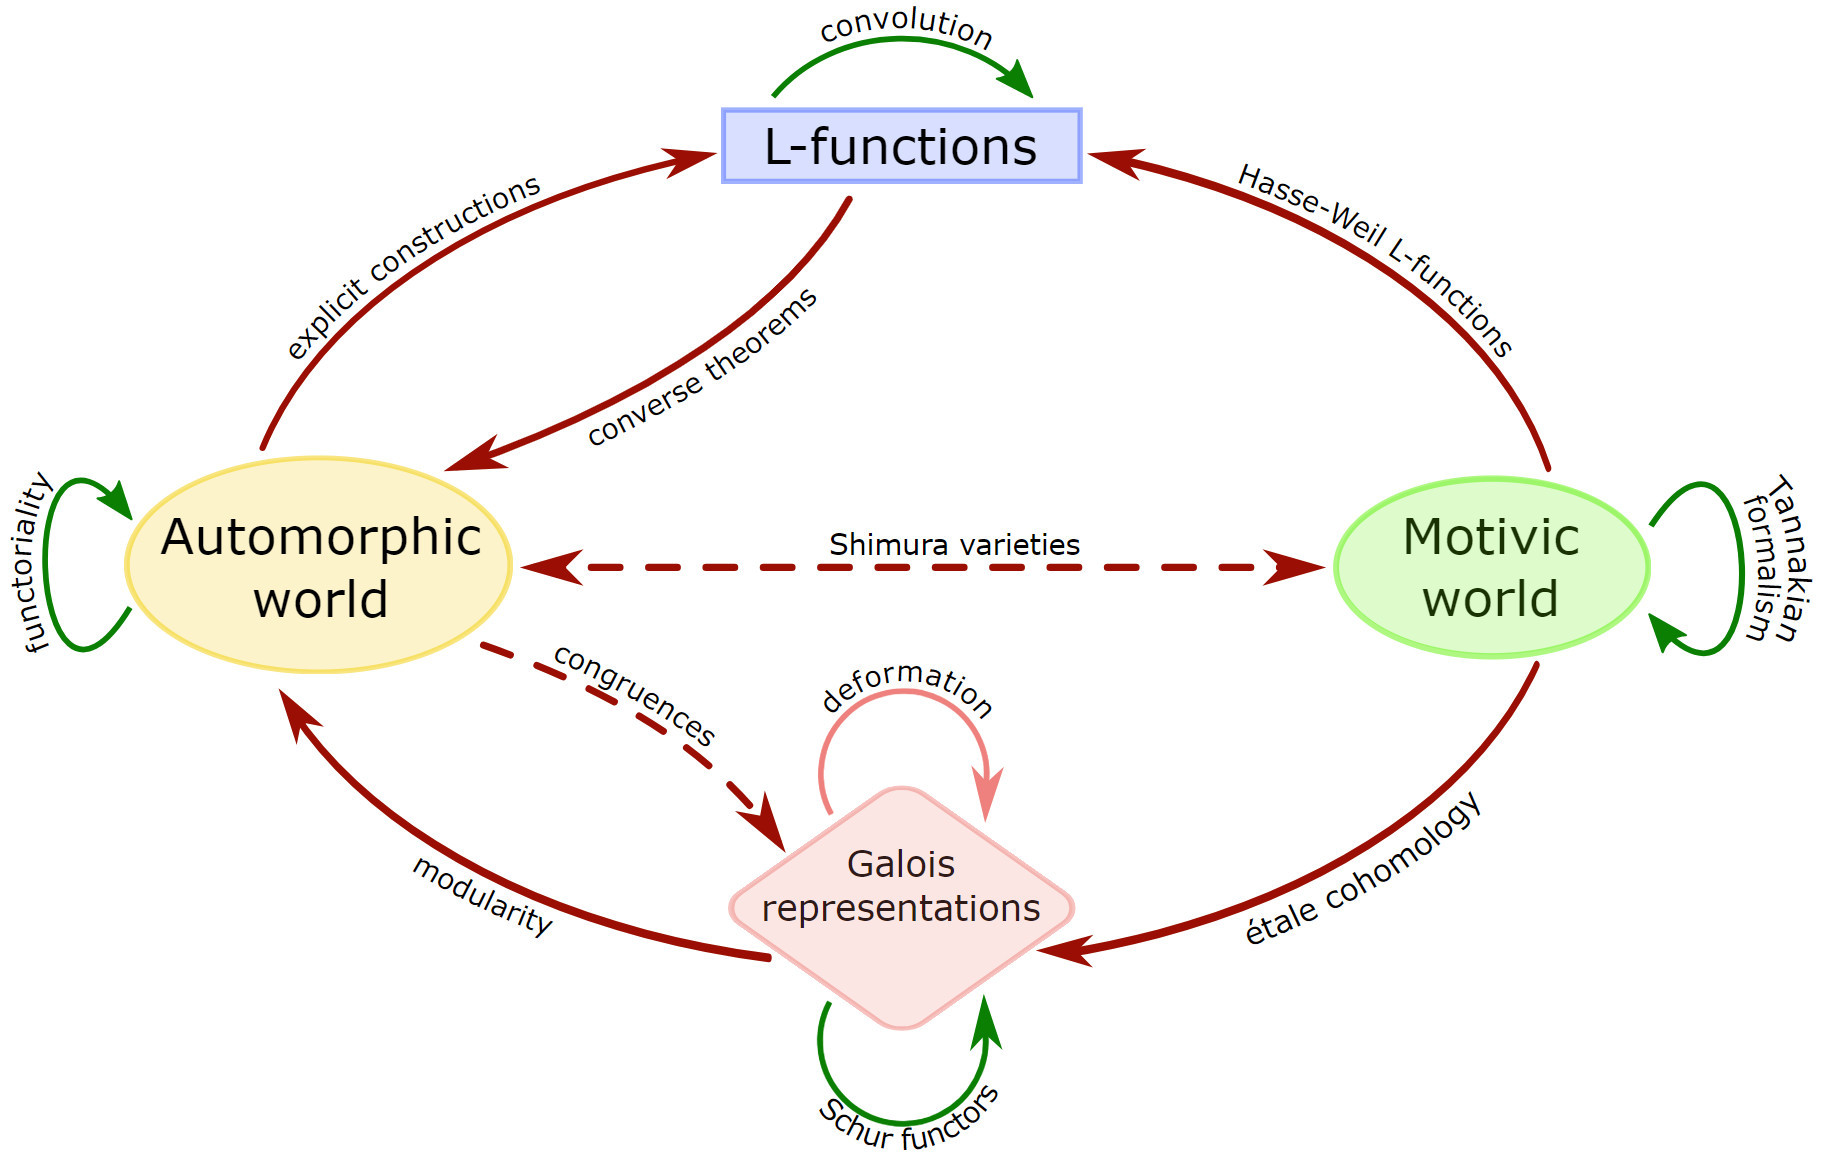
\includegraphics[scale=0.12]{LAMG.jpg}
\end{figure}

此图简要展示在不同语言下的Langlands对应关系,可以从中领略Langlands 纲领与数论,代数几何,解析理论等等学科的密切关联。
\end{frame}
\begin{frame}
\frametitle{Langlands纲领的历史背景}
其中:L函数是通过Euler乘积下的Dirichlet级数,用来研究素数密度问题,它是著名的黎曼 $\zeta$ 函数推广;自守形式领域是赋值向量环(ad\'{e}le) $G(\mathbb{A}(F))$ 在自守形式空间上的表示。在经典模形式理论会构造很多自守表示,比如Siegel形式和Maass形式;Motivic领域是指Motives是概形的上同调的和,通过他们构造绝对Motivic Galois群表示的范畴;Galois表示即为全局域上Galois群的连续表示,比如 $l$ -adic Galois表示。
\end{frame}
\begin{frame}
\frametitle{本课题的研究目标和意义}

此论文\cite{Bernshtein_1976}\footnote{I N Bernshtein and A V Zelevinskii.
Representations of the Group GL (n, F) Where F is a
Non-Archimedean Local Field.
Russian Mathematical Surveys, 31(3):1–68, jun 1976.}主要探究 $G=GL_{n}$ 时,即 $\tilde{G}=GL_{n}$时,如何将超尖表示和不可约的 $n$ 维一般线性群的表示之间的等价关系推广到更为一般的情形。
\begin{itemize}
  \item 本文中主要探究通过尖表示构造不可约表示的方法为了Langlands早期的工作提供证明技术的支持,是Langlands纲领得以诞生和推广的必要条件之一;
  \item
而对于 $GL_{n}$ 的处理,为Langlands纲领后续的发展提供必要的技术手段和理论基础,尤其目前对于高阶群的表示仍然存在着很多未知。
\end{itemize}

\end{frame}

\begin{frame}
\frametitle{继往开来}

\begin{itemize}
  \item[继往] :回顾现今数学发展一个重要的突破对于$\mathfrak{P}$-adic群表示理论是由Langlands和Jacquet在1970年出版的书籍:《Automorphic Forms on GL (2): Part 1》\cite{jacquet2006automorphic}\footnote{Herv´e Jacquet and Robert P Langlands.
Automorphic Forms on GL (2): Part 1, volume 114.
Springer, 2006.}。此书中初步的指出了这套表示论和数论之间极为漂亮的联系:即为非交换的reciprocity法则。\footnote{此书在在很多方面上奠定了表示论的研究前景。}
\item[开来] :本文探究的重点在于将其书中一些猜想性质的想法推广到$GL_{n}$的实现。对于Langlands纲领而言,仅仅 $GL_{2}$上成立是不足以称为纲领的,需要在所有情况成立,而对于 $n$ 维情况的证明的重要性是不言而喻的。

\end{itemize}

\end{frame}
\begin{frame}
\frametitle{本课题相关研究现状}
\begin{itemize}
  \item[直接相关研究] :早在1977年,Bernshtein发表系列论文:“Induced representation of $\mathfrak{P}$-adic reductive groups”\cite{ASENS_1977_4_10_4_441_0}意图进一步解决退化群的诱导表示相关的问题。对于 $\mathfrak{P}$-adic 诱导表示的高阶情况目前仍然在不断取得重要成果\cite{Vigneras2017}。
  \item[其他数学领域] :最著名的结果便是Fermat大定理的证明\cite{wiles1995modular},其中依靠着$SL_{2}$的表示证明结果。近些年Peter Scholze对于局部Langlands 纲领的几何化通过对$\mathrm{Spec}(E)$的\'{e}tale上同调和协变范畴的分析\cite{wiles1995modular},无疑正是依赖着\cite{Bernshtein_1976}的结果。
  \item[理论物理] :对于几何Langlands纲领而言,该纲领在函数域上的表示提供了二维量子场论和四维超杨-Mills流形之间的对应,其证明需要着对于圈群的表示论结果\cite{frenkel2007langlands}。
\end{itemize}

\end{frame}
\section{研究方法}

\frame{\frametitle{目录}\tableofcontents[currentsection]}

\subsection{Harish-Chandra方法}

\subsection{Gel'fand-kazhdan方法}



\begin{frame}
  \frametitle{研究方法}
首先考虑局部紧的零维的群的表示,进而用Harish-Chandra的方法来分析一般线性群 $GL_{n}$ 的表示,此方法如上文提到是尖表示诱导构造,其中对于一些有限阶的群情况下的结论早在论文\cite{Bernshtein_1976}\footnote{I N Bernshtein and A V Zelevinskii.
Representations of the Group GL (n, F) Where F is a
Non-Archimedean Local Field.
Russian Mathematical Surveys, 31(3):1–68, jun 1976.}前已经被证明,故此也不再赘述。

\vspace{0.7cm}

最后通过Gel'fand-kazhdan方法来进一步分析一般情形下的 $GL_{n}$ 的表示,这个方法与上述Harish-Chandra方法相反,是将 $GL_{n}$ 表示限制到子群 $P_{n}$ 上。
\end{frame}


% insert a reference frame before the 'thank you' frame ----------------------
\begin{frame}[allowframebreaks]
\frametitle{参考文献}
\bibliographystyle{unsrt}
\bibliography{Langlands}
\end{frame}

% Insert a thank your frame ------------------------------------------------
\begin{frame}
\frametitle{致敬}
\Huge{\centerline{Merci bien!}}

\end{frame}
\end{document} 